\chapter{Doubling the evidence: Addition of twin studies}
\label{chap:seven}

So far, I have explored the role of schooling and its contribution to an individual's future earnings. Furthermore, I tried to answer the question of what role ability plays in this equation and whether or not it should be accounted for.
Even though I claim that some magnitude of ability bias exists in the relationship, one crucial question remains unanswered. This question is - to what extent is the increase in earnings influenced by schooling and to what extent by ability? Is there a way to separate these two and isolate the effect schooling has on an individual's wage, regardless of their ability? As it turns out, there is. Using a sample of identical twins, one may theoretically rule out the role of ability and family background and observe the unbiased influence of education on earnings. In the following chapter, I attempt to take this approach by constructing an entirely new dataset containing only natural twin studies. With this dataset, I will run the analysis anew and try to determine whether individual differences and innate ability play a crucial role in determining one's future or whether it is all just a matter of education.


\section{Understanding natural experiments: Is it all intertwined?}
\label{sec:twins_literature}

For this analysis, it is vital to understand how being a twin plays a significant role in the matter. We can identify two types of twins - monozygotic and dizygotic. Monozygotic twins (marked further as MZ twins), sometimes called identical twins, come from a single zygote and thus share the same genetic information. For this, it is reasonable to assume they share the same innate ability, and any noteworthy differences that arise during their lifetime should come from their environment, schooling, family background, etc. Dizygotic twins (marked further as DZ twins), on the other hand, come from two different zygotes, and their genetic information thus differs slightly. As such, these may be looked at more as siblings of the same age. For our purposes, monozygotic twins are of particular interest, for if we subset the data to include only these, we can theoretically rule out the role of ability and family background and observe the unbiased influence of education on earnings.

Undoubtedly, this simple line of thinking has its cavetas, as there could still exist bias in the within-twin pair estimators, as pointed out, for example, by \cite{bound1999double}, or \cite{nakamuro2012estimating}. What is more, given that most of the data on twin samples comes from reported estimates, a measurement error could arise in the sample. This is well demonstrated in two of perhaps the most prominent studies in the field, \cite{ashenfelter1994estimates} and \cite{ashenfelter1998income}, where the authors construct a survey and study samples of twins to find that the \ac{OLS} estimate of returns to schooling is upward biased. In \cite{ashenfelter1994estimates}, the authors propose a new approach to combat the measurement error where the measurements of education are collected from both twins, and the final estimate comes from the within-twin comparison. This involves taking one twin's report of the within-twin schooling as an instrument for the other twin's report. The benefit of this approach lies in addressing the possible measurement error that sometimes arises in schooling reports. Several other studies, including \cite{behrman1994endowments}, \cite{isacsson1999estimates}, or \cite{bonjour2003returns}, too follow a similar approach and provide a solid theoretical background to the matter.

Another vital issue, as well as a critique of the twin approach, lies in the idea that the within-twin schooling differences may not be random but endogenous with respect to wages. \cite{bound1999double}, for example, argue that ability can be influenced by factors other than genes and that using methods such as \ac{IV} regression to remedy the measurement error can simultaneously increase the omitted ability bias. On the other hand, using techniques such as Fixed-effects estimator may remove the omitted variable bias but does so at the cost of introducing even greater bias in measurement error \citep{ning2005economic}.

For the purpose of this study, given that its main focus is to determine the extent of the omitted ability bias, I will not explore the issues of measurement error or endogeneity in the twin studies. Instead, holding the simple assumption that ability is inherently the same for identical twins, I will assume that no ability bias exists in the twin data samples. This strong assumption will allow me to directly compare the obtained results to those of the previous chapters, where the omitted ability bias was present. If I discover the results differ, it may further strengthen the notion that the omitted ability bias is indeed present in the data.


\section{What do you mean there are two?: Making a twin dataset}
\label{sec:twins_data}

I will construct the new dataset, comprising natural experiments, with two analysis goals in mind. First, as described in the previous section, I will attempt to quantify the omitted variable bias, and second, I will want to compare the results with the conclusions obtained from the earlier chapters. As such, the form of the dataset will be nearly identical to the one described in \autoref{chap:three}, with slight modifications to accommodate the specific design of the included studies.

As for the studies themselves, I start with the literature review of \cite{nakamuro2012estimating} and \cite{li2012estimating}, and from there, perform snowballing to identify as many relevant studies on the topic as possible. Using this approach, I identified, in total, 16 collectable studies. However, three of these only reported data on mixed samples (both MZ and DZ twins, or MZ twins and non-twins), so I decided to exclude them from the dataset. The remaining 13 studies, which I will use for the analysis, are listed in \autoref{app:one}.  Given how intertwined the studies on the topic are, perhaps due to the relatively small scope of the topic, the choice of which papers to include was somewhat streamlined. Possibly, I may have missed several studies, but I am highly confident that this set should provide a highly representative sample of the literature.

The most important criteria for the selection of each of these studies was for them to feature data on monozygotic twins. Given that most of the papers featured data on dizygotic twins, or non-twins subjects as well, so I decided to collect all available information. However, for the purpose of this analysis, I subset the data only to the observations that concern monozygotic twins. During the collection, it also became apparent that some variables were unusable for this particular use case. Two variables, \textit{Sector: Public/Private}, \textit{Sector: Urban/Rural}, had no observations associated with them at all, while the variables \textit{Control: Experience squared}, \textit{Control: Occupation}, and \textit{Education: Primary/Secondary/...} had fewer than ten. As such, I removed all these variables from the dataset, together with the \textit{Ability} variable, for the approach to measuring ability bias is slightly different now, as explained in \autoref{sec:twins_literature}. For some variable groups, only some sub-categories had no data, such as \textit{Estimate: Sub-region/Continent}, \textit{Micro Data}, \textit{Region: Lat-America/Middle East and North Africa/South Asia/Saharan Africa}, \textit{Income: Low}, \textit{Instrument: Distance to school}, and finally, \textit{Control: Health}. On the other hand, I also added a handful of new variables, including:

\begin{itemize}
  \item \textit{White/Non-white} - Ratio of white subjects to non-white subjects.
  \item \textit{Married/Unmarried} - Ratio of married subjects to non-married subjects.
  \item \textit{Identical/Non-identical/No twins} - Ratio of subjects that are either identical (MZ) or non-identical (DZ) twins or are not twins at all.
  \item \textit{Method: Selection/FE} - =1 if the authors use  Selection-effects or Fixed-effects estimation.
  \item \textit{Method: IV First-differenced} - =1 if the authors use First-Differenced IV estimation.
  \item \textit{Instrument: Smoking} - =1 if the authors use smoking as an instrument in the regression.
\end{itemize}



For the list of all variables used in the analysis and their descriptive statistics, see \autoref{tab:twins_new_vars}. For the list of descriptions of the rest of the variables, see \autoref{tab:var}. The final form of the new dataset includes 154 observations across 13 studies and can be found in the online appendix.

The most immediate information that can be derived from the summary statistics lies in the overall mean effect. Whilst in the main data frame, I found it to be around 7.4\%, in the data capturing only identical twin subjects, the mean effect drops down to 6.8\%, hinting at a presence of omitted ability bias. As for the other statistics, we can see that about two thirds of the subjects are married, roughly 56\% are white, and around 75\% live in high-income countries. The subjects spend, on average, around 12.4 in school and 17.8 years working. For over 90\% of them, the schooling statistic is reported in years, as opposed to levels. Other statistics, including variable groups capturing data type, estimation method, publication characteristics, etc., can all be found in the aforementioned \autoref{tab:twins_new_vars}.

\begin{table}[!htbp]
  \centering
  \scriptsize
  \singlespace
  \caption{Variables of the twin dataset}
  \label{tab:twins_new_vars}
  \begin{tabular}
    {
      @{\hskip\tabcolsep\extracolsep}
      l
      *{3}{c}
      |
      l
        *{3}{c}
      @{}
    }
    \toprule
    Variable                                                                & Mean   & SD                  & Obs   & Variable                                                               & Mean  & SD    & Obs \\
    \midrule
    Effect                                                                  & 6.819  & 3.349               & 154   & Income: Middle                                                         & 0.26  & 0.44  & 40  \\
    \multicolumn{3}{l}{\textit{\hspace{0.1cm}Estimate characteristics}}     &        & Median Expenditure  & 9.166 & 1.386                                                                  & 154                 \\
    Standard Error                                                          & 1.544  & 1.055               & 154   & Minimum Wage                                                           & 6.607 & 1.042 & 154 \\
    Estimate: City                                                          & 0.597  & 0.492               & 92    & Academic Freedom Index                                                 & 0.749 & 0.279 & 154 \\
    Estimate: Region                                                        & 0.065  & 0.247               & 10    & \multicolumn{3}{l}{\textit{\hspace{0.1cm}Estimation method}}           &                     \\
    Estimate: Country                                                       & 0.338  & 0.474               & 52    & Method: OLS                                                            & 0.26  & 0.44  & 40  \\
    \multicolumn{3}{l}{\textit{\hspace{0.1cm}Data characteristics}}         &        & Method: GLS         & 0.143 & 0.351                                                                  & 22                  \\
    Study Size                                                              & 1.304  & 0.939               & 154   & Method: Selection/FE                                                   & 0.208 & 0.407 & 32  \\
    Yrs. of Schooling                                                       & 13.061 & 0.999               & 154   & Method: FD                                                             & 0.065 & 0.247 & 10  \\
    Yrs. of Experience                                                      & 15.639 & 4.891               & 154   & Method: IV-FD                                                          & 0.104 & 0.306 & 16  \\
    Education: Years                                                        & 0.929  & 0.258               & 143   & Method: IV                                                             & 0.221 & 0.416 & 34  \\
    Education: Levels                                                       & 0.071  & 0.258               & 11    & Instr.: Sibling Ed.                                                    & 0.188 & 0.392 & 29  \\
    Wage: Hourly                                                            & 0.403  & 0.492               & 62    & Instr.: Smoking                                                        & 0.104 & 0.306 & 16  \\
    Wage: Monthly/Annual                                                    & 0.597  & 0.492               & 92    & Control: Age                                                           & 0.617 & 0.488 & 95  \\
    Survey Data                                                             & 0.909  & 0.288               & 140   & Control: Age$^2$                                                       & 0.513 & 0.501 & 79  \\
    National Register Data                                                  & 0.091  & 0.288               & 14    & Control: Experience                                                    & 0.325 & 0.47  & 50  \\
    Cross-sectional Data                                                    & 0.578  & 0.496               & 89    & Control: Ethnicity                                                     & 0.169 & 0.376 & 26  \\
    Panel Data                                                              & 0.422  & 0.496               & 65    & Control: Gender                                                        & 0.539 & 0.5   & 83  \\
    Data Year                                                               & 3.300  & 0.863               & 154   & Control: Marriage                                                      & 0.539 & 0.5   & 83  \\
    \multicolumn{3}{l}{\textit{\hspace{0.1cm}Spatial/Structural variation}} &        & Control: Firm Char. & 0.097 & 0.297                                                                  & 15                  \\
    Wage Earners                                                            & 0.913  & 0.062               & 32    & Control: Area                                                          & 0.039 & 0.194 & 6   \\
    Gender: Male                                                            & 0.429  & 0.231               & 129   & Control: Macro Var.                                                    & 0.071 & 0.258 & 11  \\
    Gender: Female                                                          & 0.571  & 0.231               & 25    & \multicolumn{3}{l}{\textit{\hspace{0.1cm}Publication characteristics}} &                     \\
    White                                                                   & 0.573  & 0.444               & 87    & Impact Factor                                                          & 0.139 & 0.86  & 110 \\
    Ethnicity: Caucasian                                                    & 0.201  & 0.402               & 31    & Citations                                                              & 3.844 & 2.357 & 124 \\
    Married                                                                 & 0.679  & 0.155               & 88    & Study: Published                                                       & 0.714 & 0.453 & 110 \\
    Unmarried                                                               & 0.321  & 0.155               & 66    & Study: Unpublished                                                     & 0.286 & 0.453 & 44  \\
    Income: High                                                            & 0.74   & 0.44                & 114   & Publication Year                                                       & 1.383 & 0.743 & 130 \\

    \bottomrule
    \multicolumn{8}{>{\scriptsize}p{0.9\linewidth}}{\emph{Note:} This table presents basic summary statistics for variables of the new twin dataset. Some variables are omitted for the sake of brevity. For detailed descriptions of all variables unmentioned in this chapter, see \autoref{tab:var}. For values of the omitted variables, see the source twin dataset in the appendix. SD = Standard Deviation, OLS = Ordinary Least Squares, GLS = Generalized Least Squares, FE = Fixed-Effects, IV = Instrumental Variable.}
  \end{tabular}
\end{table}

\section{Empirical analysis: Are the results just identical?}
\label{sec:twins_analysis}

To determine whether the returns to educations are different for identical twins, and to what extent if so, I will employ the same methods as in the previous chapters. The main focus will be on the effect size, which is assumed to be unbiased by ability in the twin dataset. First, I include several graphs that allow us to glance into the data to spot any immediate patterns. For these, see the subsection below. Second I take another look the publication bias models explained in \autoref{chap:four}, and whether or not they yield different results in the context of natural studies. These results can be found in \autoref{tab:PB-Twins}.

\subsection*{Graphical patterns and immediate takeaways}

First, in \autoref{fig:funnel_plot_twins}, I present the funnel plot, as described in \autoref{chap:four}. As a reminder, the plot should show the data symmetrically distributed around the mean in case of no publication bias. For our purpose, this will allow us to determine the behavior of the data after the ability bias is accounted for, and see whether we can spot any obvious changes in said bevaior.

To complement the funnel plot, I also present a box plot in \autoref{fig:box_plot_twins}, which displays estimates of all studies in the twin dataset, clustered at study level. This plot will allow us to see the distribution of the data from another perspective, and spot any outliers that may be present.


\begin{figure}[!htbp]
  \begin{center}
    \caption{The twin studies funnel plot}
    \label{fig:funnel_plot_twins}
    \begin{subfigure}[b]{0.45\textwidth}
      \caption{All observations}
      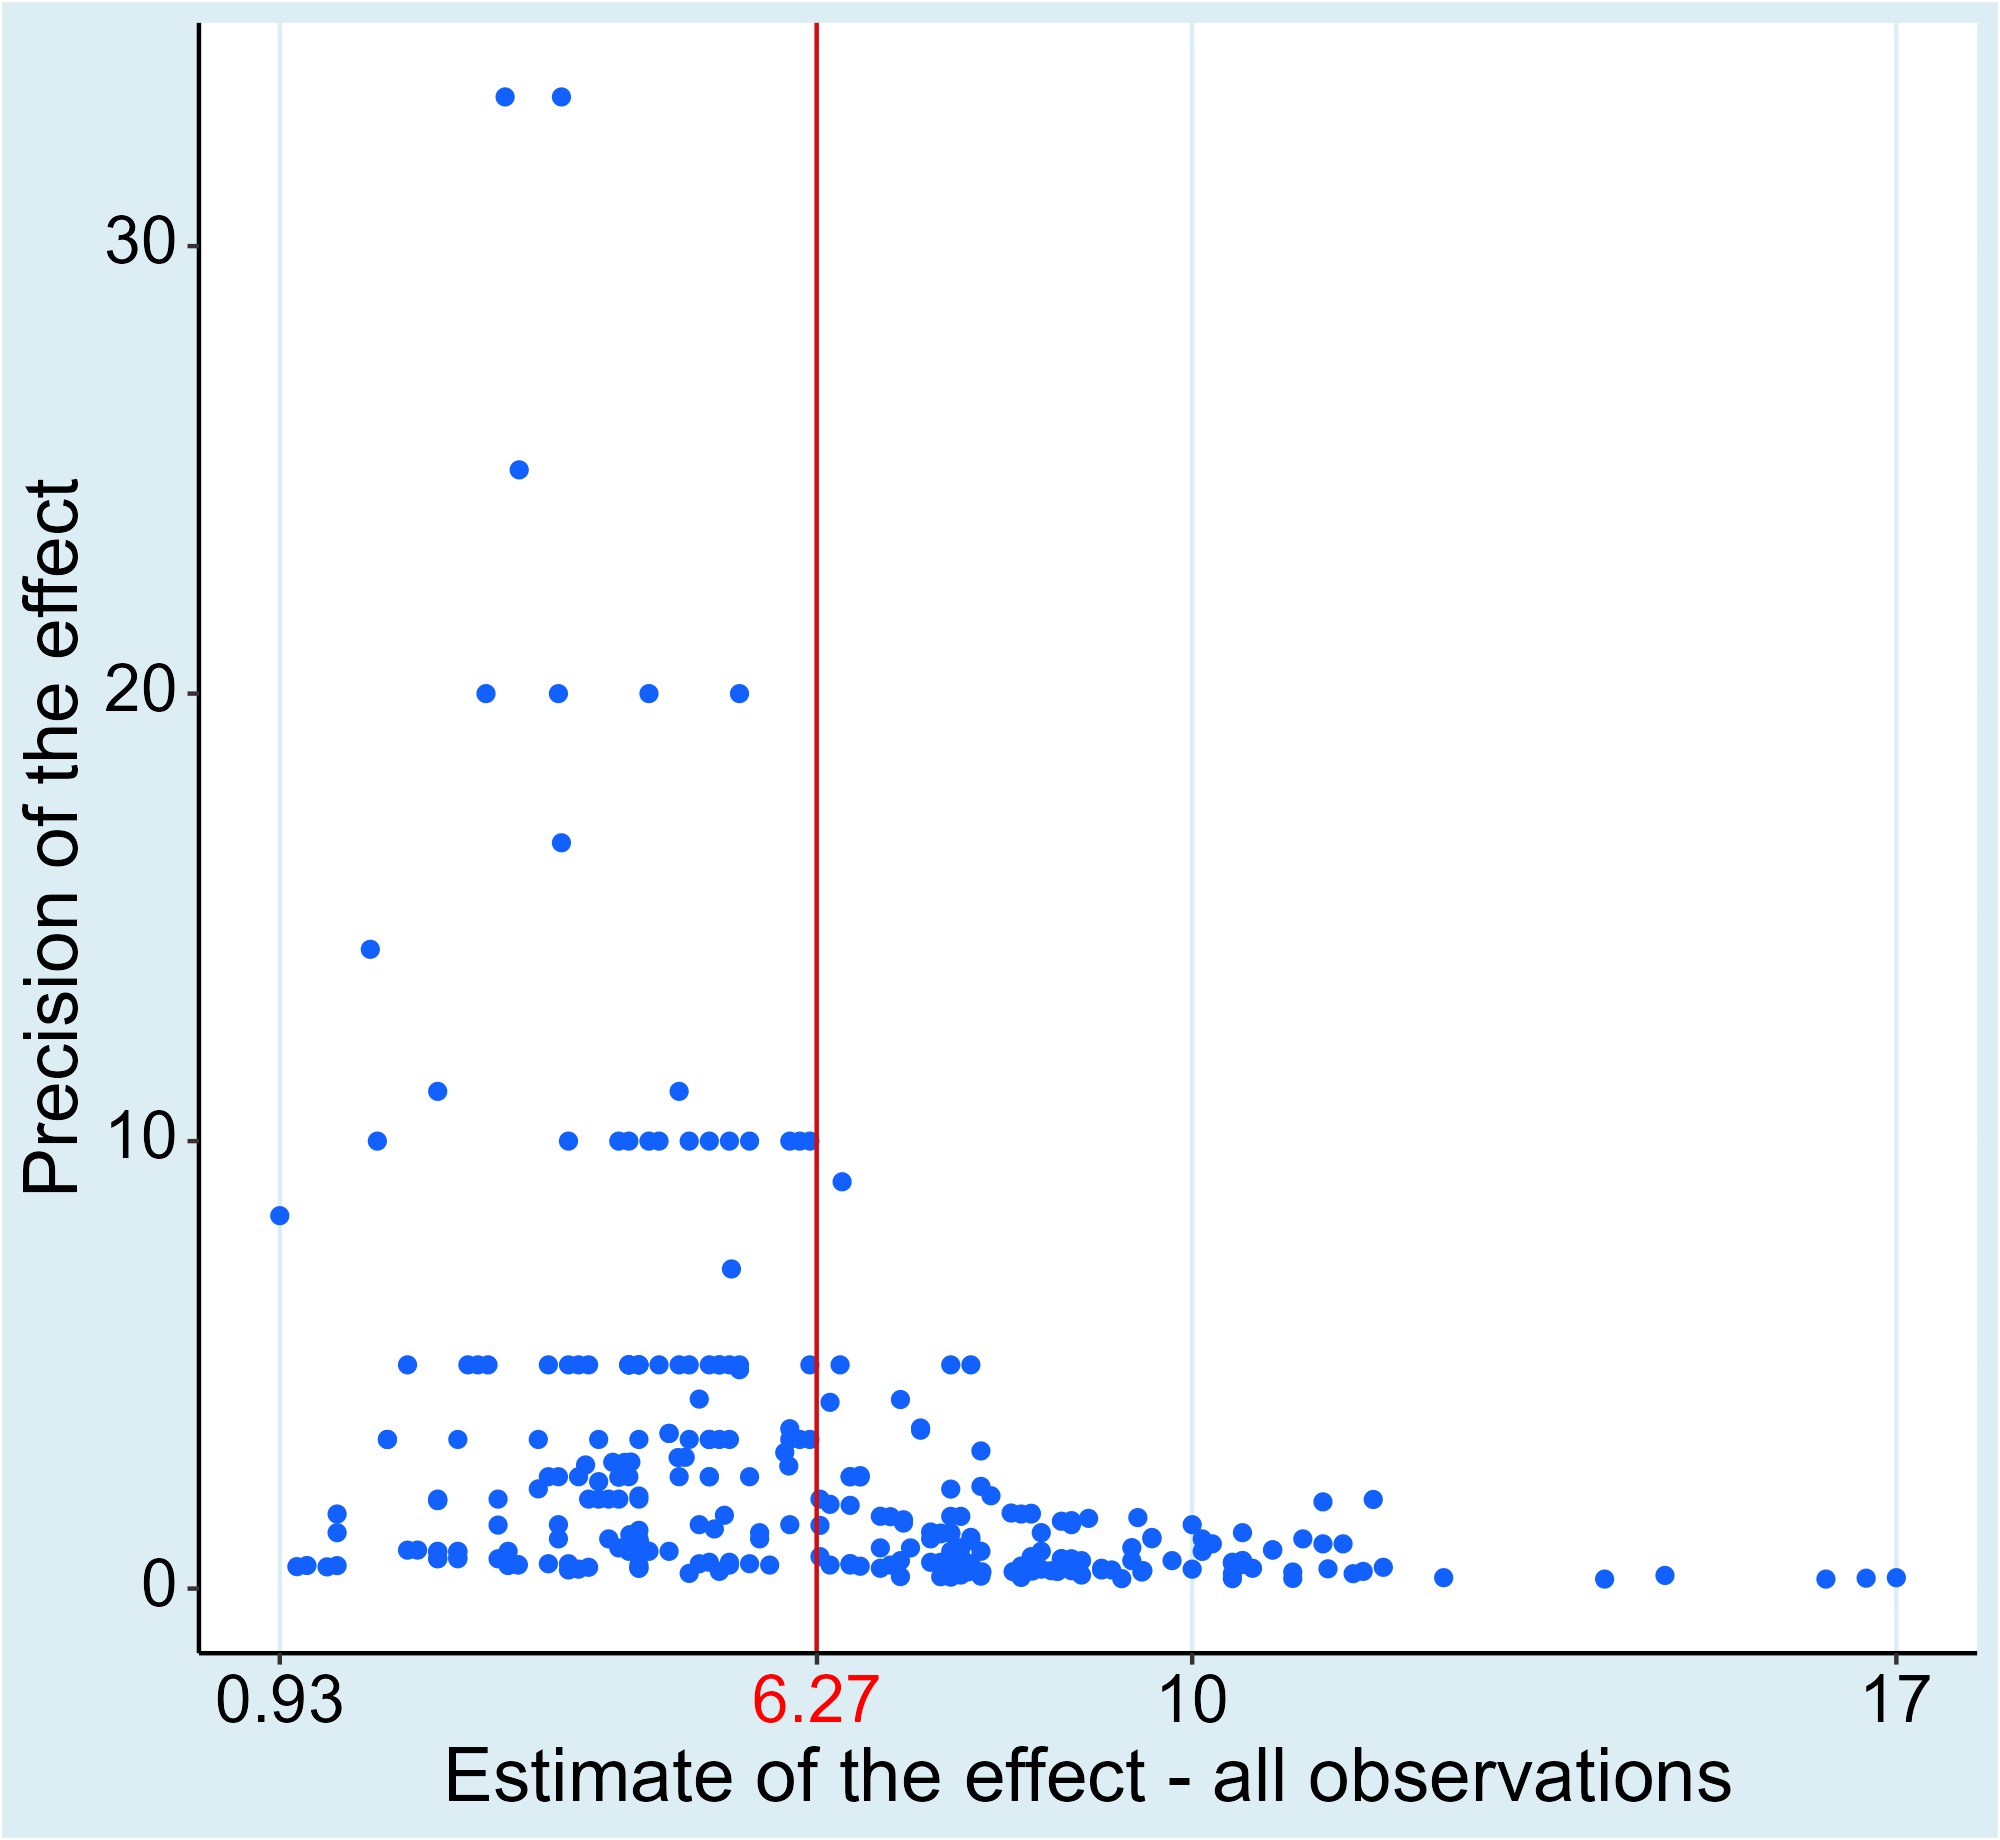
\includegraphics[width=0.95\linewidth]{Figures/funnel_twins.png}
      \label{fig:funnel_plot_twins_all}
    \end{subfigure}
    \begin{subfigure}[b]{0.45\textwidth}
      \caption{Study medians}
      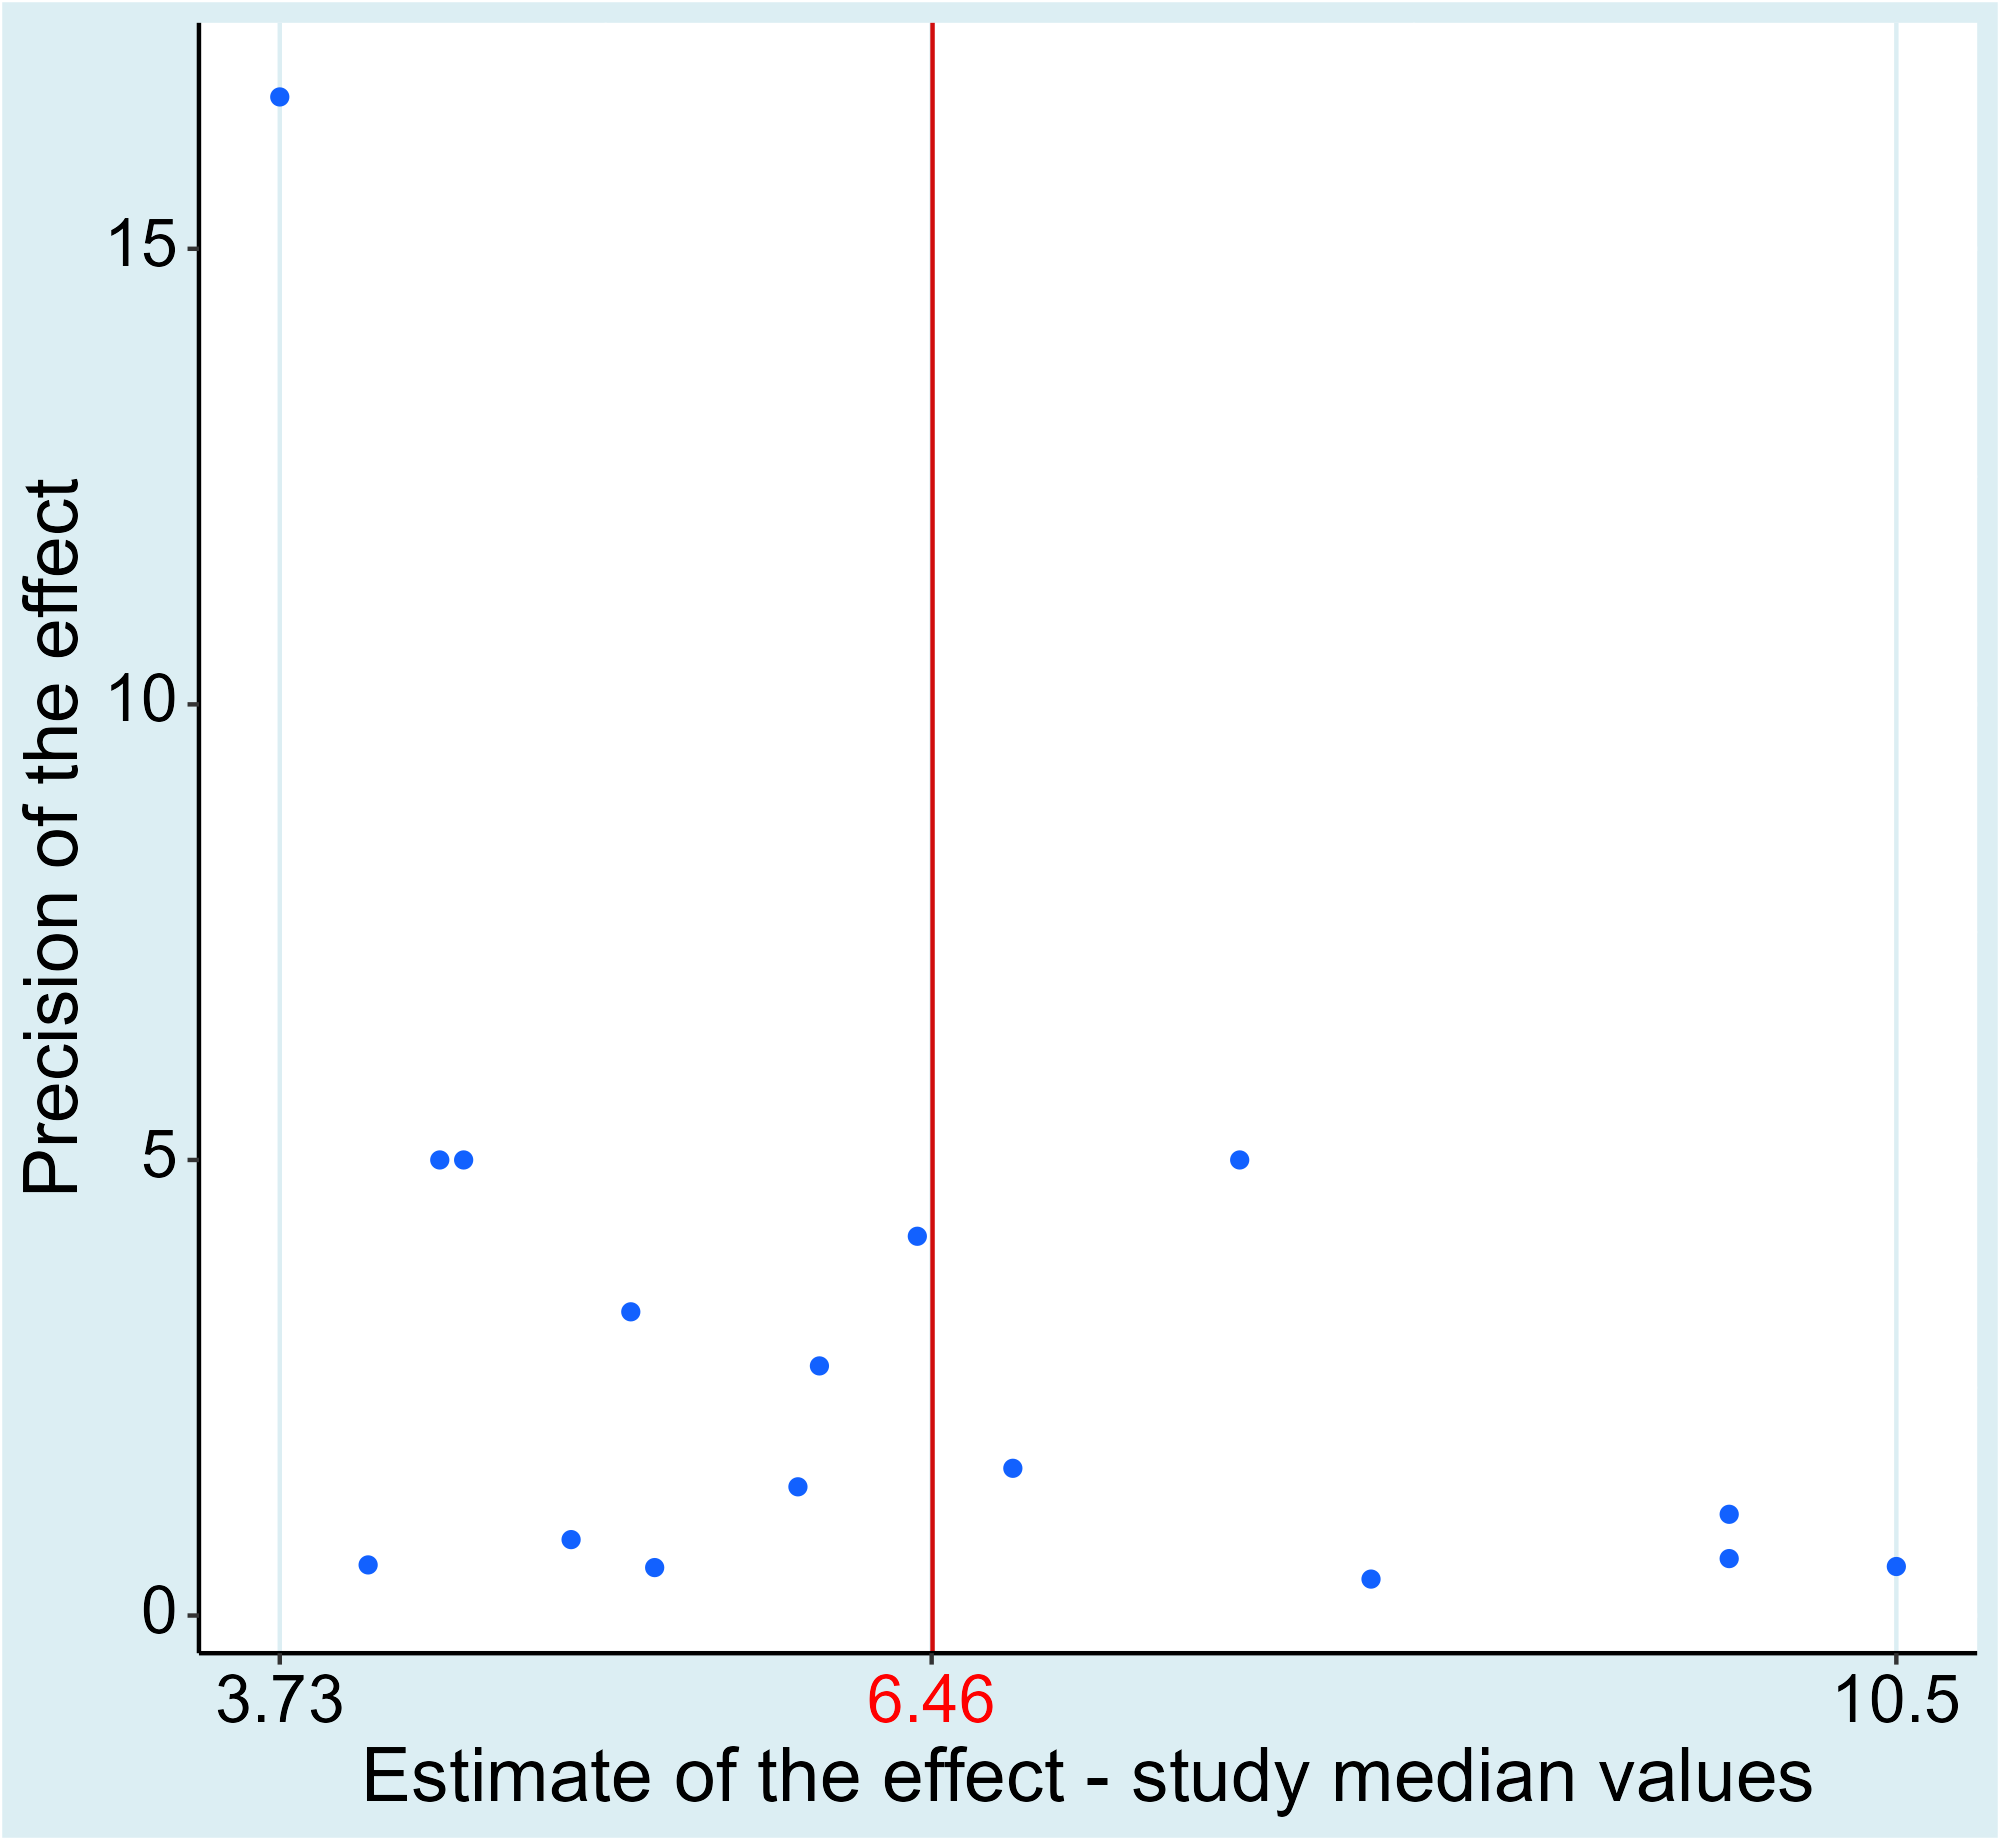
\includegraphics[width=0.95\linewidth]{Figures/funnel_twins_medians.png}
      \label{fig:funnel_plot_twins_medians}
    \end{subfigure}
  \end{center}\vspace{-0.6cm}
  \captionsetup{width=0.85\textwidth, font = scriptsize}
  \caption*{\emph{Note:} This figure displays two funnel plots as per \cite{Egger1997}, where the percentage returns to an additional year of schooling are plotted on the x-axis against precision on the y-axis, measured as $1/SE$ (Standard Error). Plot (a) shows the funnel plot for all observations within the twin data (154 data points), while plot (b) shows only the medians of each study (13 data points). The red line marks the mean of these data points. In case of no publication bias, these funnel plots should be symmetrically centered around the true mean.}
\end{figure}


\begin{figure}[!htbp]
  \begin{center}
    \caption{Box plot of estimates natural studies}
    \label{fig:box_plot_twins}
    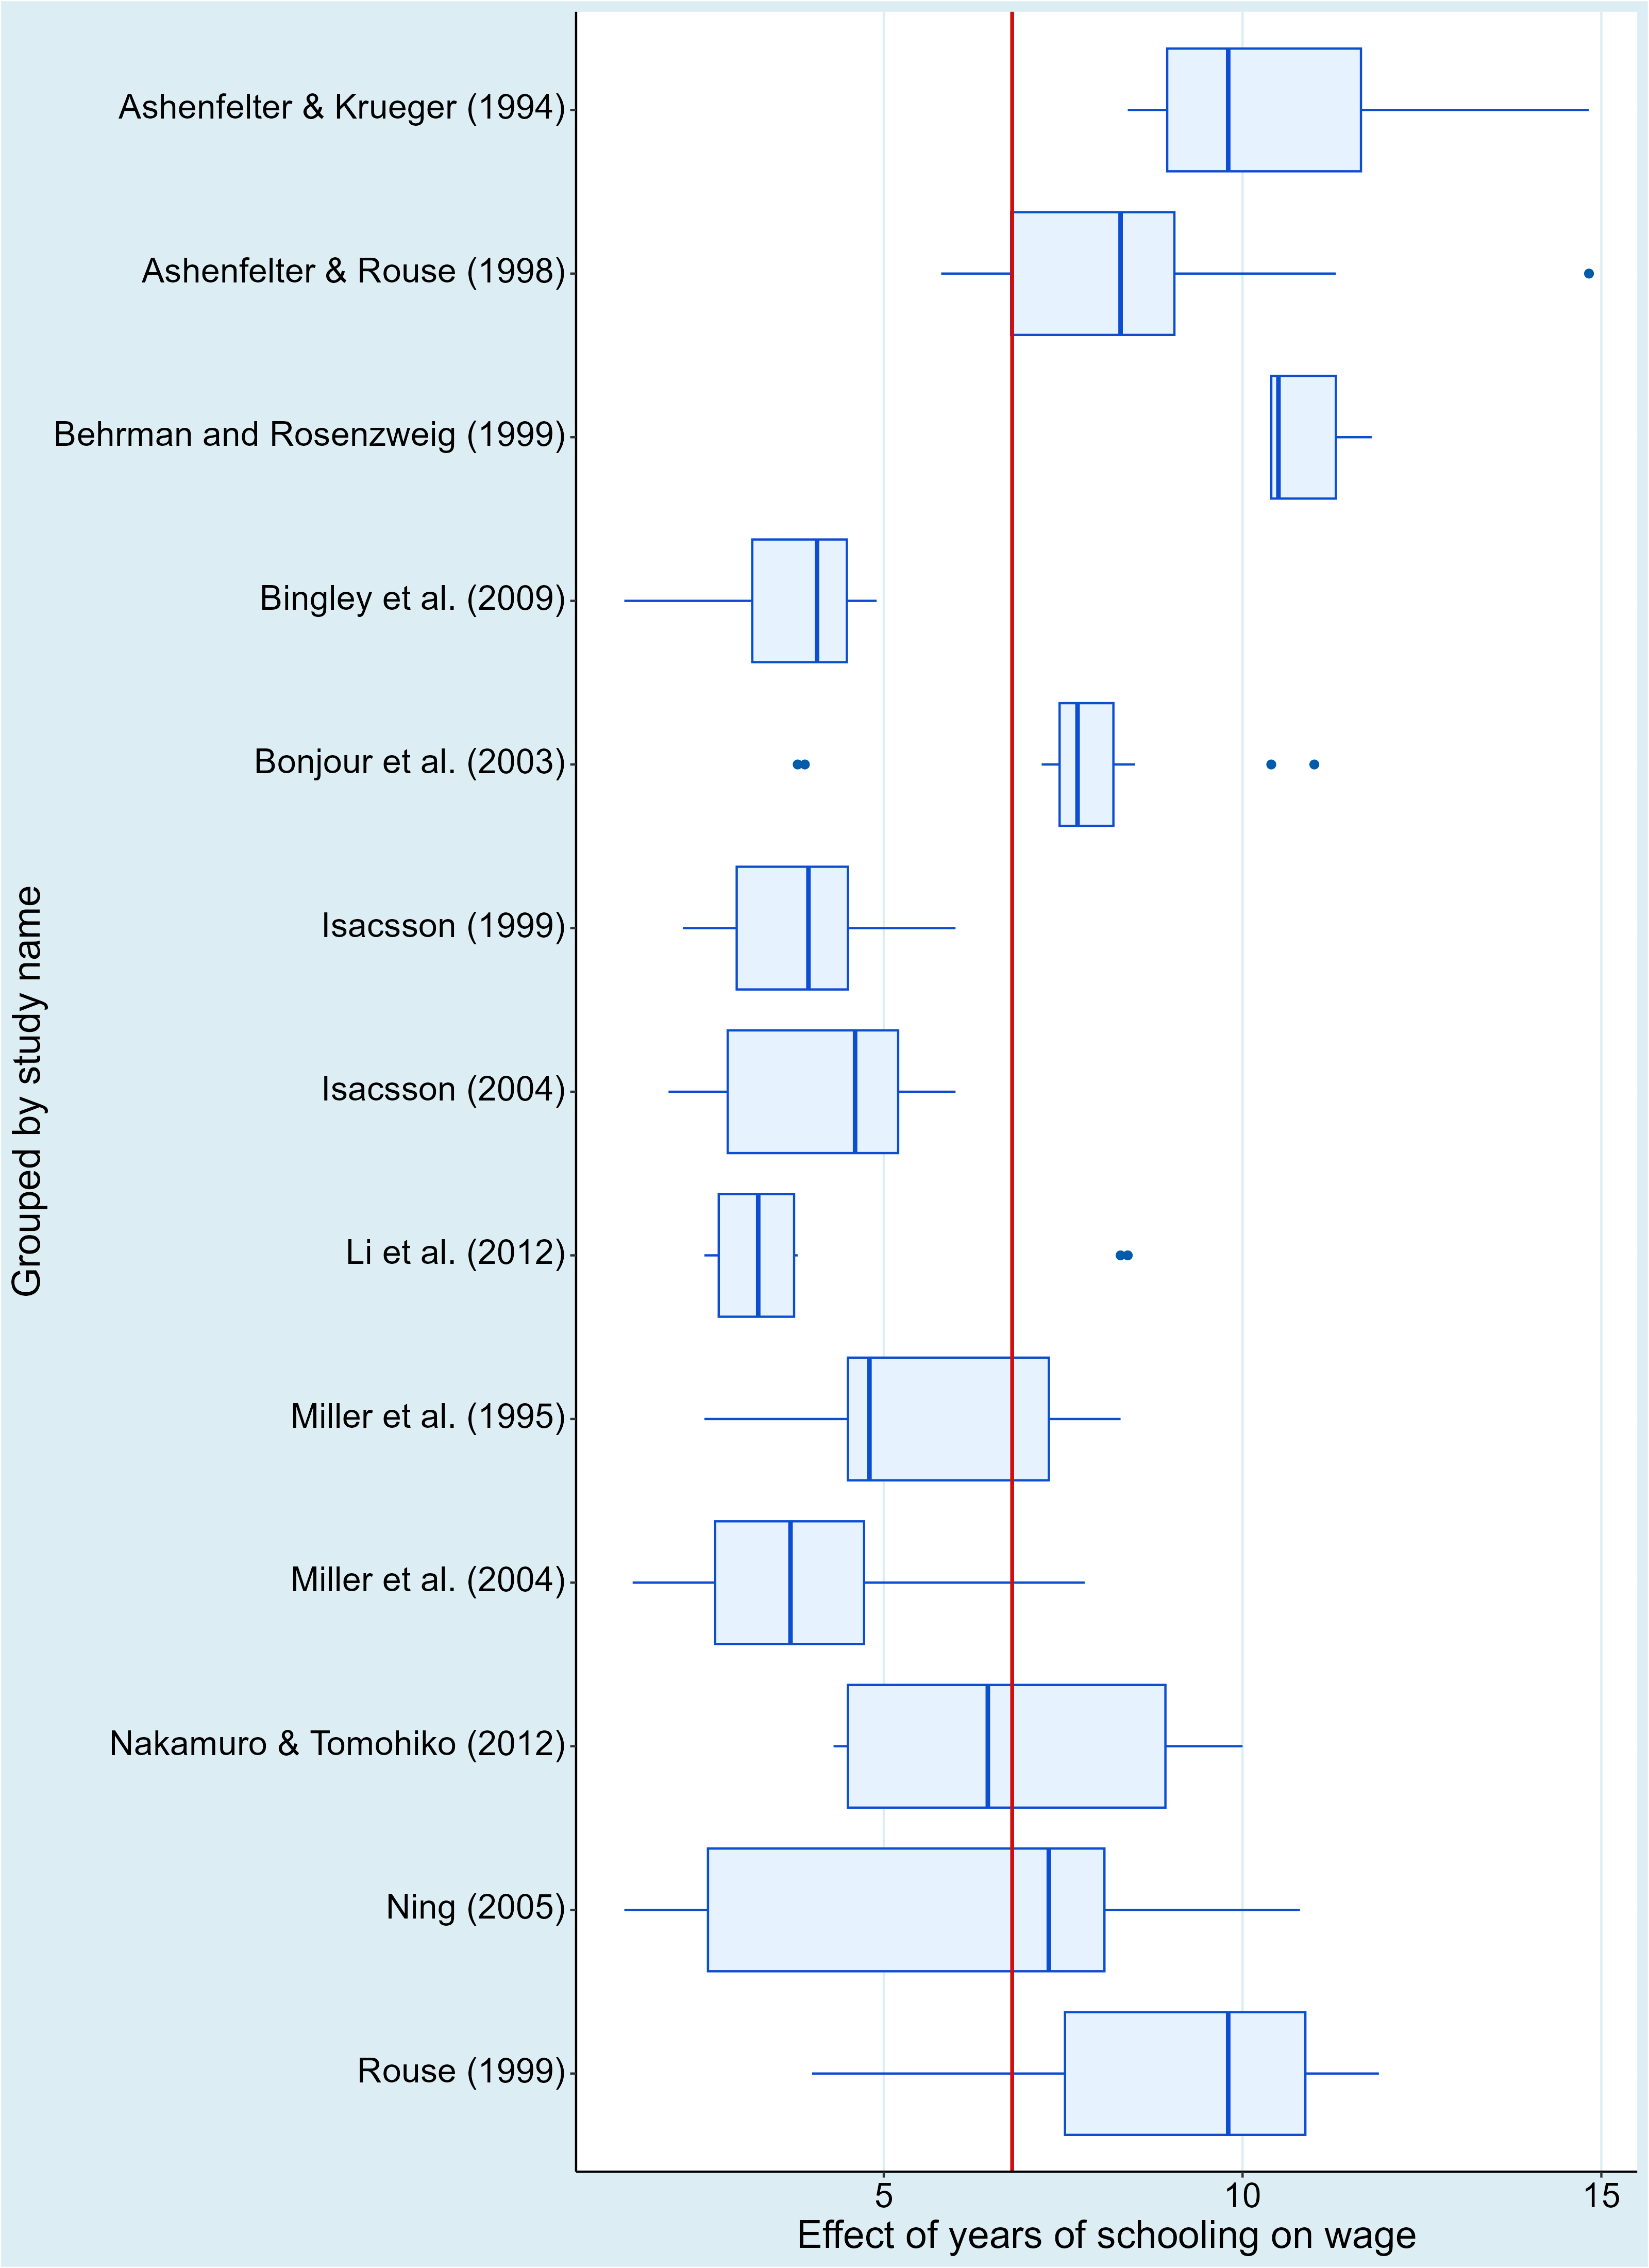
\includegraphics[width=0.9\textwidth]{Figures/box_plot_study_name_twins.png}
  \end{center}\vspace{-0.7cm}
  \captionsetup{width=0.9\textwidth, font = scriptsize}
  \caption*{\emph{Note:} This plot shows a box plot for data of the twin dataset, where the esimates are grouped at the study level. The red line represents the average effect across the literature. Each box's length represents the interquartile range between the 25th and 75th percentiles. The dividing line within each box indicates the median value. The whiskers extend to the highest and lowest data points within 1.5 times the range between the upper and lower quartiles. Outliers are depicted as blue dots. The red line depicts the mean of the effect within the data. The data is winsorized at 1\% level.}
\end{figure}

The funnel plots in \autoref{fig:funnel_plot_twins_all} both tell a similar story - the overall effect tends to be lower than in the case of the main dataset. Moreover, the data points are not symmetrically distributed around the mean, but rather skewed to the right. This suggests that the publication bias is present in the twin dataset, and that the effect of schooling on earnings is likely overestimated.


The box plot in \autoref{fig:box_plot_twins} further supports this notion, although not as clearly. While most of the studies report effects that are lower than the mean, there are several outliers that report higher effects. This is in line with the funnel plot, where a non-negligible number of estimates appear above the mean, although their precision is not high enough to be considered significant. Peculiarly, the studies of \cite{ashenfelter1994estimates} and \cite{ashenfelter1998income} report the highest effects, which may be due to the measurement error in the data, as discussed in \autoref{sec:twins_literature}. Given my simplistic assumptions about the dataset, that aim to isolate the effect of schooling from ability bias, many other effects are sure at play here that may influence the results. This includes the aforementioned measurement error, together with endogeneity, and other biases that may arise in the twin studies.


\subsection*{Twin studies and publication bias}

Next I take a quick look at the size of returns to schooling when treated for both the ability bias and for publication bias in a rigorous manner. Here, similarly to \autoref{chap:four}, I will utilize a battery of tests, including linear and non-linear methods, as well as methods that relax the exogeneity assumption. Given that I could not hope, nor intend to include all models listed in \autoref{chap:four}, I will focus on the core battery, including OLS, Fixed Effects, Random Effects, WAAP, Top10, Stem, AK, Kink, IV, and p-uniform*. The results of these tests can be found in \autoref{tab:PB-Twins}.

% Linear tests
\begin{table}[!htbp]
  \centering
  \small
  \singlespace
  \caption{Twin studies and publication bias}
  \label{tab:PB-Twins}
  \begin{tabular}{
      @{\hskip\tabcolsep\extracolsep}
      l*{5}{c}} %one left column, five center (*{} makes the cols inherit attributes)
    \toprule
    \multicolumn{6}{l}{\textit{Panel A: Linear methods}}                                            \\
    \multicolumn{1}{c}{}                  &
    \textbf{OLS}                          &
    \textbf{FE}                           &
    \textbf{RE}                           &
    \textbf{Study}                        &
    \textbf{Precision}                                                                              \\
    \midrule

    Publication bias                      & 1.306*** & 0.369*** & 2.497*** & 0.620*** & 2.486***    \\
    \emph{\hspace{0.2cm}(Standard error)} & (0.209)  & (0.231)  & (0.737)  & (0.226)  & (0.459)     \\
    \addlinespace[0.5em]
    Effect beyond bias                    & 4.776*** & 6.221*** & 3.126*** & 5.681*** & 3.714***    \\
    \emph{\hspace{0.2cm}(Constant)}       & (0.399)  & (0.403)  & (1.130)  & (0.571)  & (0.393)     \\
    \addlinespace[0.5em]
    Observations                          & 154      & 154      & 154      & 154      & 154         \\


    \midrule

    \multicolumn{6}{l}{\textit{Panel B: Non-linear methods}}                                        \\
                                          &
    \textbf{WAAP}                         &
    \textbf{Top10}                        &
    \textbf{Stem}                         &
    \textbf{AK}                           &
    \textbf{Kink}                                                                                   \\
    \midrule
    Publication bias                      &          &          &          & 2.912*** & 2.486***    \\
                                          &          &          &          & (0.157)  & (0.436)     \\
    \addlinespace[0.5em]
    Effect beyond bias                    & 6.212*** & 4.576*** & 4.263*** & 6.037    & 3.714***    \\
                                          & (0.280)  & (0.441)  & (0.490)  & (NA)     & (0.142)     \\
    \addlinespace[0.5em]
    Observations                          & 154      & 154      & 154      & 154      & 154         \\

    \midrule

    \multicolumn{6}{l}{\textit{Panel C: Methods relaxing the exogeneity assumption}}                \\
    \multicolumn{4}{c}{}                  &
    \textbf{IV}                           &
    \textbf{p-uniform*}                                                                             \\
    \midrule
    Publication bias                      &          &          &          & 2.191*** & L = 1.205   \\
                                          &          &          &          & (0.275)  & (p = 0.272) \\
    \addlinespace[0.5em]
    Effect beyond bias                    &          &          &          & 3.409*** & 7.658       \\
                                          &          &          &          & (0.505)  & (NA)        \\
    \addlinespace[0.5em]
    Observations                          &          &          &          & 154      & 154         \\

    \bottomrule
    \multicolumn{6}{>{\footnotesize}p{0.95\linewidth}}{\emph{Note:} Panel A: Results obtained from estimating the linear equation \autoref{eq:fat_reg}. Standard errors, clustered at the study level, are included in parentheses. OLS = Ordinary Least Squares. FE = Fixed Effects. RE = Random Effects. Precision = Estimates are weighted by the inverse of their standard error. Study = Estimates are weighted by the inverse number of observations reported per study. Panel B: Estimates of the effect and publication bias using five non-linear methods. WAAP = Weighted Average of the Adequately Powered \citep{Ioannidis2017Waap}, Top10 = Top10 method by \cite{Stanley2010Top}, Stem = the stem-based method by \cite{Furukawa2019Stem} where P represents the probability of results insignificant at 5\% are published relative to the probability of the significant ones at the same level, AK = \cite{Andrews2019Selection}'s Selection model, Kink = Endogenous kink model by \cite{Bom2019Kink}. Standard errors, clustered at the study level, are included in parentheses. Panel C: Estimates of the effect and publication bias using two techniques that relax the exogeneity assumption. IV = Instrumental Variable Regression; the inverse of the square root of the number of observations is used as an instrument for the standard error. Standard errors, reported in parentheses, are also clustered at the study level. P-uniform* = method proposed by \cite{vanAert2021puni}; L represents the publication bias test t-statistic, the corresponding p-value can be found in parentheses. ***p<0.01, **p<0.05, *p<0.1}
  \end{tabular}
\end{table}

A clear takeaway from these tests, which holds across different methods and approaches, is that publication bias is present and prominent in the twin dataset. Further yet, if we look at the effect beyond bias, which represents here returns to schooling after ability bias and publication bias are accounted for, we can see that the effect drops even further, on average by roughly two to three percentage points. To be concrete, the STEM-based method suggests returns to education of 4.2\%, while the Endogenous Kink approach claims 3.7\%. On the other end of the spectrum, \ac{WAAP} and the Selection model report the highest returns, 6.2\%, and \%, respectively, which still lower than the dataset average effect of 6.8\%. In fact, the only method that suggests a coefficient of returns toschooling higher than the simple data average is p-uniform*, where we have no information on the standard error, and thus significance.

All in all, all checks presented here suggest that the returns to schooling are lower than previously estimated, and that the omitted ability bias is indeed present in the data. Accounting for this bias, the returns to schooling drop by roughly 2-3 percentage points, which is a significant decrease.